\documentclass[conference]{IEEEtran}

\usepackage{cite}
\usepackage{amsmath,amssymb,amsfonts}
\usepackage{algorithmic}
\usepackage{graphicx}
\usepackage{textcomp}
\usepackage{xcolor}
\def\BibTeX{{\rm B\kern-.05em{\sc i\kern-.025em b}\kern-.08em
    T\kern-.1667em\lower.7ex\hbox{E}\kern-.125emX}}
\begin{document}

\title{Addressing the $p \gg n$ Problem: A Study of Model Efficacy using Maize Flowering Time Prediction}

\author{\IEEEauthorblockN{Gabriel Guillen}
\IEEEauthorblockA{\textit{dept. of Statistics \& Data Science} \\
\textit{University of Central Florida}\\
Orlando, United States of America \\
ga013701@ucf.edu}}


\maketitle

\begin{abstract}
This study aims to evaluate and compare $p \gg n$-compatible statistical models for predicting Maize Flowering Time within a high-dimensional setting. The objective is to identify the modeling method that delivers the optimal trade-off among predictive accuracy, model robustness against overfitting, and practical computational efficiency in handling large-scale data. This analysis will inform the selection of robust and efficient methods for a high-dimensional problem.\\
\end{abstract}

\section{\textbf{Introduction}}
\indent This report evaluates the efficacy of specialized statistical methodologies against a high-dimensionality genomic dataset for the prediction of Maize Flowering Time (dtoa). Traditional statistical approaches are inherently unsuitable for this problem setting, defined by the \textbf{$p \gg n$} regime where the number of predictors ($p$) vastly outnumbers the observations ($n$).\\
\indent A key consequence of high dimensionality is the instability of variance, which compromises the reliability and confidence of model performance due to an elevated risk of overfitting. Therefore, the chosen models must incorporate regularization and feature selection to stabilize estimates and identify true signals. \\
\indent The core objective of this analysis is to determine which modeling method provides the optimal balance of predictive accuracy and robustness given compute time when faced with this complex, high-dimensional structure. \\

\subsection{\textbf{Dataset Structure}}
\indent The dataset \cite{buckler2009} consists of $4,981$ observations ($n$) and $7,390$ variables ($p$), including some amount of missing data. The dependent variable is Time to Male Flowering (\texttt{dtoa}). The independent variables are predominantly $7,389$ Single Nucleotide Polymorphism (SNP) markers ($m_1-m_{7389}$), supplemented by $25$ (1-25) categorical variables representing the genetic crosses or families (\texttt{pop}). \\

\section{\textbf{Methods}}

\subsection{\textbf{Data Preparation}}

\subsubsection{\textbf{Preprocessing}}
\indent Initial data cleaning involved the \textit{removal of incomplete observations}; specifically, any row containing one or more missing values was excluded from the effective dataset. This procedure reduced the total number of records from $4,981$ to $4,494$. \\
\indent The resulting data loss, approximately $10\%$  of the original sample, was deemed acceptable given the scope and objectives of this analysis. Following this cleaning step, the $4,494$ retained observations were \textit{randomly partitioned} into three distinct subsets for model development and evaluation. \\
\indent The subsets were allocated as follows: $75\%$ ($\approx 3,371$ records) for the \textit{training set}, $15\%$ ($\approx 674$ records) for the \textit{validation set}, and the remaining $10\%$ ($\approx 449$ records) for the final, unbiased \textit{test set}. This division ensures a rigorous assessment of model performance and generalization capabilities. \\
\subsubsection{\textbf{Standardization}}
\indent To prepare the data for models designed to handle high-dimensionality, all features were subjected to \textit{standardization}, often referred to as $Z$-score normalization. This critical preprocessing step transformed each feature such that its distribution had a mean of zero ($\mu=0$) and a standard deviation of one ($\sigma=1$). Mathematically, this transformation is defined as $z = (x - \mu) / \sigma$. \\
\indent This procedure ensures that all features are centered around zero and scaled to unit variance, a step essential for promoting \textit{equitable contribution} from every feature during the model's learning process. \\

\subsection{\textbf{High-Dimensionality Regression Models Used}}

\begin{enumerate}
	\item \textbf{Stepwise Regression}: In particular the forward algorithm, this technique builds a model by iteratively adding or removing predictors based on a statistical metric, retaining only the most significant features. It works in $p \gg n$ scenarios by drastically reducing the effective number of predictors, thus avoiding the computational and statistical pitfalls of a full model.
	\item \textbf{Lasso Regression}: Lasso adds an $\ell_1$ penalty (absolute value of coefficients) to the model, which forces the coefficients of less important features to become exactly zero. This automatically performs crucial feature selection, making it excellent for $p \gg n$ by providing a sparse, interpretable model.
	\item \textbf{Ridge Regression}: Ridge adds an $\ell_2$ penalty (squared value of coefficients) to the model, which shrinks all coefficients towards zero but never sets them to exactly zero. This effectively stabilizes the model and mitigates the high variance and multicollinearity issues common in $p \gg n$ datasets.
	\item \textbf{Elastic Net Regression}: Elastic Net combines both the $\ell_1$ (Lasso) and $\ell_2$ (Ridge) penalties in its objective function. It leverages the feature selection ability of Lasso while maintaining the stability of Ridge, making it robust for complex high-dimensional data with highly correlated predictors.
	\item \textbf{Principal Component Regression (PCR)}: PCR first uses Principal Component Analysis (PCA) to transform the original $p$ features into a smaller set of uncorrelated latent components (composite variables). It then runs an ordinary linear regression on these few components, completely solving the $p \gg n$ problem by moving to a much lower-dimensional space.
	\item \textbf{Partial Least Squares Regression (PLS)}: PLS constructs new latent variables that not only explain the variance in the predictors but also maximize their correlation with the response variable ($\mathbf{Y}$) or \texttt{dtoa} in this case. This method is effective in $p \gg n$ because its dimension reduction is supervised and specifically optimized for predictive power.\\
\end{enumerate}

\subsection{\textbf{Tuning and Selection}}

\indent All models, specifically \textbf{Lasso}, \textbf{Ridge}, \textbf{Elastic Net}, \textbf{PCR}, and \textbf{PLS}, underwent hyperparameter optimization using \textit{$k$-fold cross-validation} applied exclusively to the \textit{training set}.\\
\indent For PCR and PLS, the optimal number of components ($k$) was searched across the grid $\{5, 10, 50, 100, 200, 300, 400, 500\}$ using $k=5$ folds. In contrast, the \textbf{Stepwise Regression} model utilized the Bayesian Information Criterion (BIC) as its selection metric due to BIC's stringent penalty on model complexity. \\
\indent The optimal hyperparameters for the \textbf{Lasso}, \textbf{Ridge}, and \textbf{Elastic Net} models can be observed in Table \ref{tab:hyperparameters}.

\begin{table}[h]
	\centering
	\caption{Hyperparameter Grid for Regularized Regression Models}
	\label{tab:hyperparameters}
	\begin{tabular}{|c|c|c|c|}
		\hline
		\textbf{Grid Index} & \textbf{Lasso ($\alpha$)} & \textbf{Ridge ($\alpha$)} & \textbf{Elastic Net ($\alpha$, $l\_ratio$)} \\
		\hline
		1 & $0.001$ & $0.0001$ & $0.001, (0.1, 0.5, 1.0)$ \\
		2 & $0.0031622777$ & $0.001$ & $.01, (0.1, 0.5, 1.0)$ \\
		3 & $0.01$ & $0.01$ & $0.1, (0.1, 0.5, 1.0)$ \\
		4 & $0.0316227766$ & $0.1$ & $1.0, (0.1, 0.5, 1.0)$ \\
		5 & $0.1$ & $1.0$ & $10.0, (0.1, 0.5, 1.0)$ \\
		6 & $0.316227766$ & $10.0$ & \texttt{n/a} \\
		7 & $1.0$ & $100.0$ & \texttt{n/a} \\
		8 & $3.1622776602$ & $1000.0$ & \texttt{n/a}\\
		9 & $10.0$ & $10000.0$ & \texttt{n/a} \\
		\hline
	\end{tabular}
	\begin{flushleft}
		\small Note: $\alpha$ is the regularization strength; $l\_ratio$ (L1 ratio) is the mixing parameter, where $0 < l\_ratio \leq 1$.
	\end{flushleft}
\end{table}

\section{\textbf{Results}}

Analysis of the tuned models yielded distinct optimal configurations, as detailed in Table \ref{tab:performance}.

\begin{table}[h]
	\centering
	\caption{Performance and Compute Time}
	\label{tab:performance}
	\begin{tabular}{|l|c|c|c|c|}
		\hline
		\textbf{Method} & \textbf{RMSE (CV)} & \textbf{RMSE (Test)} & \textbf{\# Feats / Comps} & \textbf{Time (s)} \\
		\hline
		Ridge  & 3.526 & 3.533 & 7390 & 136.914\\
		Lasso & 3.358 & 3.387 & 82 & 1214.324\\
		Elastic Net & 3.347 & 3.389 & 309 & 2026.851\\
		Stepwise (BIC) & 3.372 & 3.404 & 17 & 431.755\\
		PCR ($k$ comps) & 3.542 & 3.593 & 50 & 141.986\\
		PLS ($k$ comps) & 3.645 & 3.670 & 10 & 2927.664\\
		\hline
	\end{tabular}
\end{table}

 \indent For \textbf{Stepwise Regression}, the final model included $17$ features, selected in forward order: \{\texttt{pop}, \texttt{m439}, \texttt{m6493}, \texttt{m2419}, \texttt{m5808}, \texttt{m1652}, \texttt{m772}, \texttt{m290}, \texttt{m2548}, \texttt{m4940}, \texttt{m2969}, \texttt{m2865}, \texttt{m4772}, \texttt{m2162}, \texttt{m2276}, \texttt{m2358}, \texttt{m6665}\}. \\
 \indent The regularized models achieved maximum performance with the following hyperparameters: \textbf{Ridge} utilized a strong penalty of $\alpha=10000.0$; \textbf{Lasso} achieved optimal results at $\alpha=0.1$, resulting in a sparse model with $82$ non-zero coefficients; and \textbf{Elastic Net} also optimized at $\alpha=0.1$ with an $\ell_1$ ratio of $0.5$ (leading to $309$ non-zero coefficients). \\
 \indent Among the dimension reduction techniques, \textbf{PLS} performed best with $10$ components, while \textbf{PCR} achieved its optimal fit using $50$ components. \\
 
 \indent Across all models evaluated, the observed \textbf{Root Mean Square Error (RMSE)} from the cross-validation (CV) set was consistently lower than that of the independent test set, confirming expected model behavior and indicating a degree of generalization error common in predictive modeling. \\ \indent While the time component reported in Table \ref{tab:performance} is machine-dependent and thus serves primarily as a reference, the training times for the more complex models were substantial, often extending into the $40$-minute range given the computational resources employed.

\section{\textbf{Discussion}}

\subsection{Models Performance}

 \indent A comparison of predictive metrics, visually represented in Figure \ref{Tc_q2_rmse}, confirms that the \textbf{Lasso} and \textbf{Elastic Net} models achieved the superior performance, exhibiting the lowest prediction error, as indicated by a $\text{RMSE}$ value of approximately $3.40$, and the highest predictive power, with $\text{Q}^2$ values near $0.145$. \\ \\
\begin{figure}[htbp]
	\centerline{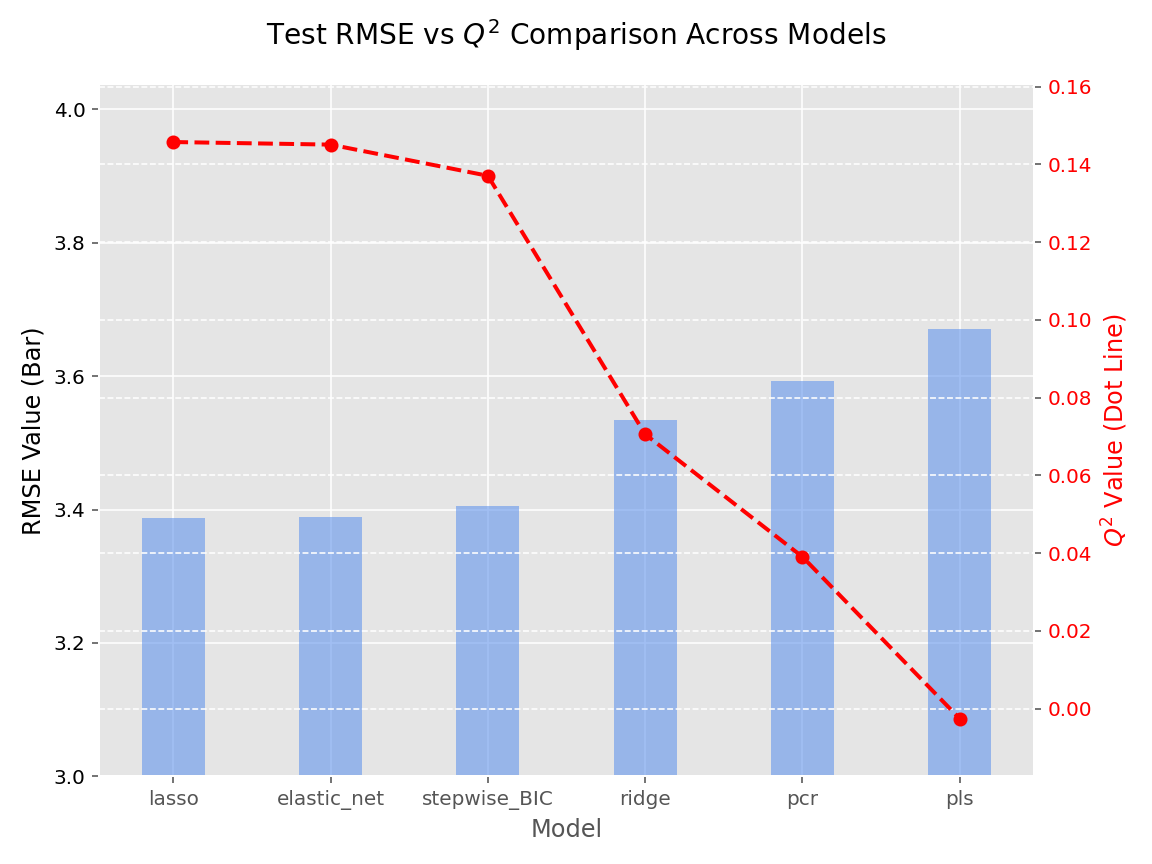
\includegraphics[scale=0.45]{test_q2_vs_rmse_barchart.png}}
	\caption{Comparing $\text{Q}^2$ against $\text{RMSE}$}
	\label{Tc_q2_rmse}
\end{figure}
 \indent Conversely, the \textbf{PLS} model performed the worst, recording the highest $\text{RMSE}$ ($\approx 3.68$) and the lowest predictive power ($\text{Q}^2 < 0.00$). \\ \\ \\ \\ \\ \\ \\ \\
 \indent While the range of $\text{RMSE}$ values across all models was narrow ($3.40$ to $3.68$), the $\text{Q}^2$ metric clearly distinguished the superior predictive ability of the sparse regularization techniques (Lasso and Elastic Net). \\

 \indent As illustrated in Figure \ref{Tc_rmse_mae}, revealed that although the $\text{RMSE}$ and \textbf{Mean Absolute Error ($\text{MAE}$)} values were numerically close across all six models ($\text{RMSE}$ clustered between $3.4$ and $3.7$; $\text{MAE}$ between $2.6$ and $2.9$), their ratio provided a key distinction.

\begin{figure}[htbp]
	\centerline{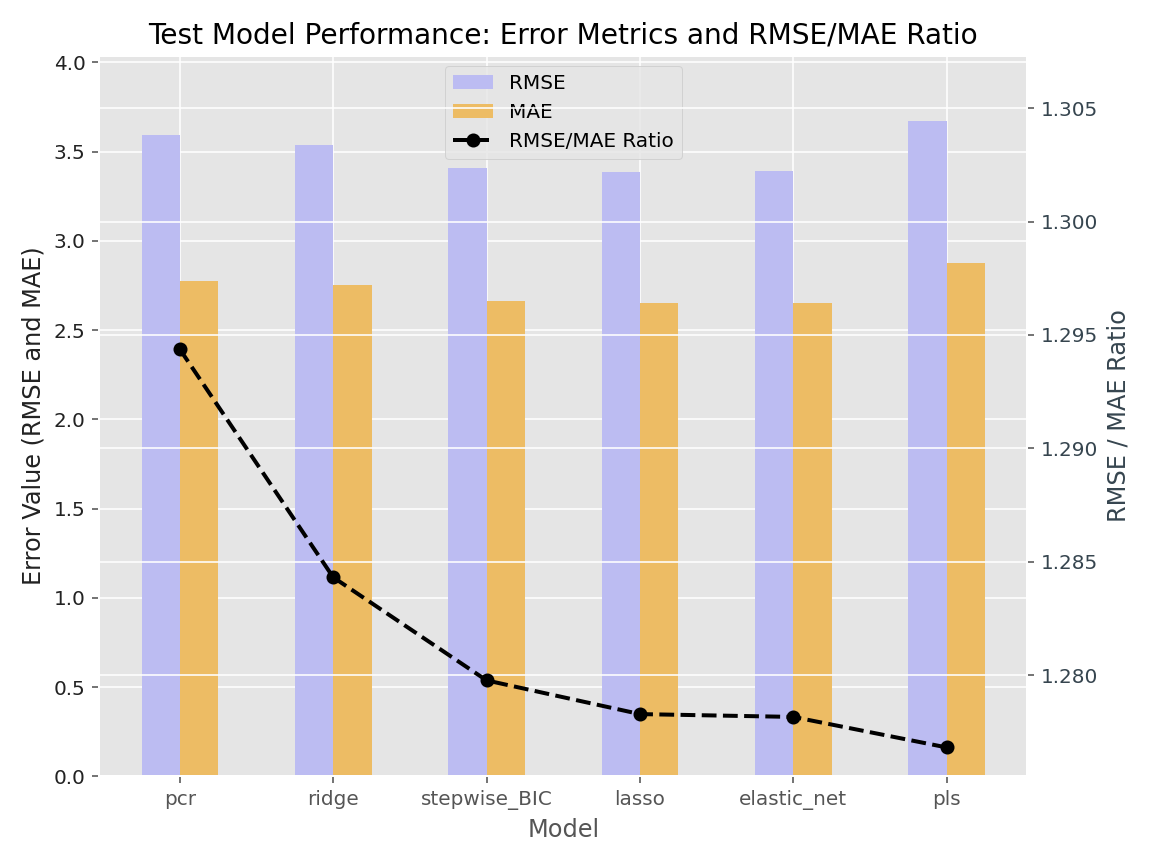
\includegraphics[scale=0.45]{test_rmse_mae_ratio_barchart.png}}
	\caption{Comparison of Regression Model Error and Ratio}
	\label{Tc_rmse_mae}
\end{figure}

 \indent \textbf{$\text{RMSE}/\text{MAE}$ ratio} demonstrated a clear decreasing trend, ranging from $\approx 1.295$ for the \textbf{PCR} model down to $\approx 1.275$ for the \textbf{PLS} model. \\
 \indent This lower ratio for \textbf{PLS} suggests that, relative to the other models, the \textbf{PLS} approach minimized the influence of large outlier errors, indicating a more robust and uniform error distribution.\\

\subsection{Accuracy-Time-Interpretability Tradeoff}

\begin{figure}[htbp]
	\centerline{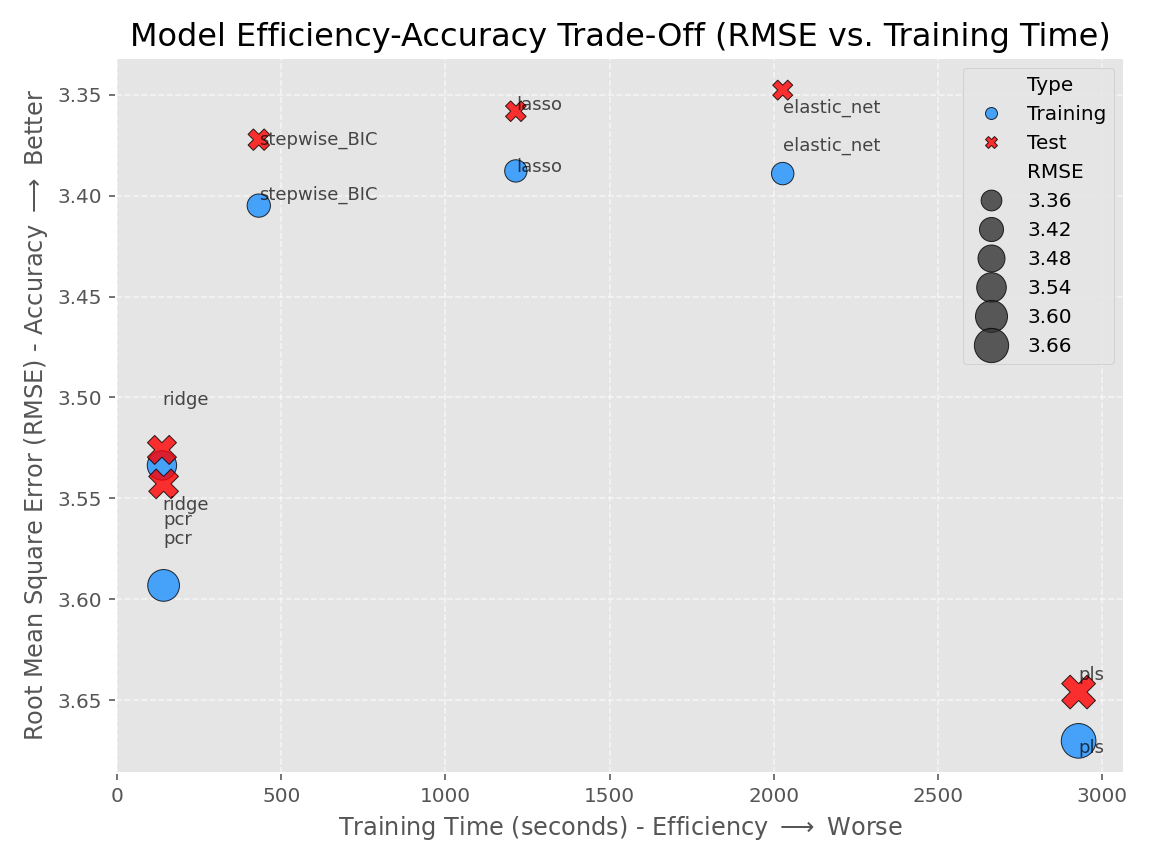
\includegraphics[scale=0.45]{rmse_and_time_scatterplot.png}}
	\caption{Model Efficiency-Accuracy Trade-Off}
	\label{Tc_time_rmse}
\end{figure}

 \indent An analysis of the predictive accuracy versus training time, visualized in Figure \ref{Tc_time_rmse}, suggests a strong connection between model sparsity and overall performance.\\
 \indent The \textbf{Stepwise Regression} model provided the most balanced solution, achieving near-best accuracy with relatively low training time, making it the most efficient choice.\\
 \indent While the \textbf{Lasso} and \textbf{Elastic Net} models yielded the highest accuracy (lowest test $\text{RMSE} \approx 3.35-3.40$), they incurred the second and third longest training times, respectively. Conversely, \textbf{Ridge} and \textbf{PCR} demonstrated the fastest training times but were not competitively accurate. \\
 \indent The \textbf{PLS} model performed the worst overall, exhibiting both the longest training duration and the lowest predictive performance.\\

\section{\textbf{Conclusion(s)}}

\indent This study concludes that the \textbf{Lasso} and \textbf{Elastic Net} models provide the optimal trade-off between \textbf{predictive accuracy} and \textbf{computational efficiency}. These methods successfully generated \textbf{sparse and effective} models.\\
\indent While \textbf{Stepwise selection} is relatively fast (efficient training), it consistently yielded slightly lower accuracy than the top-performing Lasso and Elastic Net.\\
\indent The \textbf{dimension reduction} techniques, Partial Least Squares (PLS) and Principal Component Regression (PCR), were generally less competitive. Contrary to typical assumptions, \textbf{PCR} demonstrated superior performance over \textbf{PLS} in both accuracy and training speed. The \textbf{Ridge} model offered intermediate performance and was not deemed useful in this context.\\
\indent In summary, \textbf{Lasso or Elastic Net} are the recommended models for robust predictive performance. \textbf{Stepwise selection} should only be favored when \textbf{training time is the absolute critical constraint}.

\section*{\textbf{Appendix}}
	
\section*{Appendix A: Supplementary Materials and Software Usage}
\subsection*{Source Code Repository \label{app:code}}
The source code, data, and detailed implementation scripts for this project are available on GitHub (URL: https://github.com/gaguillen4384-dev/Data-Science/tree/main/DataMining\_1/Project\_2).

\subsection*{Software Usage Acknowledgment}
The text and documentation were edited and refined using Google Gemini.

\begin{thebibliography}{9} % '9' is for formatting the numbering (up to 9 items)
	
\bibitem{buckler2009}
Buckler et al. (2009). Science 325, 714--718. (Original maize flowering time study)

\bibitem{waldmann2013}
Waldmann, P., Mészáros, G., Gredler, B., Fuerst, C., \& Sölkner, J. (2013).
Evaluation of the lasso and the elastic net in genome-wide association studies.
\textit{Frontiers in Genetics}, 4, 270.

\bibitem{hastie2009}
Hastie, T., Tibshirani, R., \& Friedman, J. (2009/2017).
\textit{The Elements of Statistical Learning} (PCR/PLS chapters).
	
\end{thebibliography}

\vspace{12pt}

\end{document}
